%----------------------------------------------------------------------------
\chapter{Mobile Robot Design}\label{chap:mobile_robot_chapter}
%----------------------------------------------------------------------------

The mobile platform performed the task of transporting the LEGO bricks between the dispenser unit, and the robot cell. It had to be able to fulfill this task in a completely autonomous manner under normal operation, avoid collision with obstacles, be harmless to its operators and be remotely controllable through a human machine interface. It was also a requirement that its progress should be monitored through the aforementioned user interface. 

Due to the high complexity of the task, we decided to pursue a modular approach. In this chapter we will introduce the components comprising the system, the motivation for having them, their implementation and the reasons behind the choices we made during the design process.



% Please keep sections separated in their designated folders and only reference them here using the input tag

%!TEX root = ../../../main.tex
\section{Frobomind} % (fold)
\label{sec:mr_frobomind}

\textbf{Someone}

A shord tesciptiotion of FroboMind, what it is, the benefit of using it in comparison to a purely ROS based system, and how we use it now...

	\subsection{Frobomind interface} % (fold)
	\label{sub:mr_frobomind_interface}
	The frobomind interface is in charge of transform the hardware sensors values into ROS messages that can be used by the user.
	This is implemented as a ROS package given inside of the frobomind framework.
	A small modification in this package has been made so the status of the battery can be read.
	This allows the robot to create subrutines of charging when needed and continuing with the previous task when charged.
	% subsection frobomind_interface (end)
% section frobomind (end)


%!TEX root = ../../../main.tex
%%---------------------------------------------------------------------------
\section{Mobile Robot Navigation \label{sec:navigation_sec}}
%%---------------------------------------------------------------------------

How the mobile robot navigates in general (system overview), and the discussion of its subsystems in details (why, how, how well):
\begin{itemize}
    \item Navigation Controller
    \item In-box navigation
    \item Out-of-box navigation
    \item Line following
    \item QR-code reading
    \item HMI
\end{itemize}
\subsection{In-box Navigation} \label{sec:in_box_navigation}
As per project description, the navigation inside the box is to be done based on SLAM. Due to complexity of the entire project and potential diversity of SLAM implementations, an open-source implementation of SLAM was chosen. More specifically the gmapping-package \cite{gmapping} which has a livid community of supporters and builds a ROS wrapper for “OpenSlam's Gmapping”\cite{openslam}. TF-Frames of Lidar, IMU and the robot base were set up, this allows for easy transformation between Lidar and odometry data, inside the package. Using these, the SLAM-Implementation uses a particle filter to sequentially build up a map of the area. By manually driving through the entire workspace, a map was created. 
\begin{figure}[H]
	\centering
	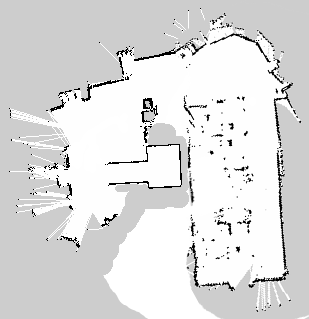
\includegraphics[width=0.5\textwidth]{slam_map}
	\caption{Slam Map}
	\label{fig:slam_map}
\end{figure}
Using the map-server package from the ROS 2D-Navigation Stack \cite{navigation_stack} the generated map was stored and is then broadcasted as a static map for localization. The AMCL (Adaptive Monte-Carlo Localization) package (which is also included in the navigation stack) then uses the static map, the lidar as well as odometry data to localize the robot while in free navigation. After tuning the parameters, AMCL worked fairly reliably for navigation both inside and outside the box.\\
\textbf{TODO: Describe move{\_}base}\\
Due to the box being fairly monotone in respect to the Lidar readings (clean, walls, no landmarks), precise navigation inside the box was sometimes not perfect. Also with multiple robots present in the box, issues, especially when trying to charge occurred. To ensure reliability of charging, a backup behaviour was added, when the charging failed using move{\_}base. For this a line was added, using the already implemented Line Following behaviour. The move{\_}base is used to navigate the robot to the start of the charging line. Then the robot follows the line until a pre-specified distance from the wall using Lidar. Having a main and a backup behaviour proved to be sufficient for reliable charging\\
\textbf{TODO: IS THAT REALLY SO?}
%!TEX root = ../../../main.tex
%%---------------------------------------------------------------------------
\section{Tipper Control \label{sec:tipper_sec}}
%%---------------------------------------------------------------------------

Description of the tipper controller. (Why, how)

%!TEX root = ../../../main.tex
\section{Safety system} % (fold)
\label{sec:mr_safety_system}
The safety in the mobile robot is intrinsic in all the nodes that allow its movement.
Additionally the Safety Eyes was supposed to be used to detect humans in the area close to the stairs. However due it not working, it was not being used.
There then are two aspects to talk about: (1) the \textbf{incident handler} based on the the given frobomind implementation. Based on certain inputs, an \emph{activation} signal is created, allowing the robot to move.
(2) On the other hand, the \textbf{obstacle detector} is used to feed another skill (see section \ref{sub:skills}) that changes the speed, or even stops, the robot depending on the distance of obstacles detected by the LIDAR.
This can be activated or disabled depending on the situation.
	\subsection{Incident handler} % (fold)
	\label{sub:mr_incident_handler}
	The incident handler is based in the \emph{simple incident handler} given inside of the frobomind framework.
	This system receives two signals: (1) the \emph{deadman} and (2) the \emph{critical fault}.
	When both signals are received correctly, the incident handler outputs another signal that \emph{enables the actuation}.
	This signal is directly received from the system that actually performs the actions that move the motors in the robot.
	Both signals are booleans with a time stamp and need two conditions to be approved:
	\begin{enumerate}
		\item As booleans, need to be true.
		\item As stamped, need to be received in an interval smaller than a threshold. In our system the signal need to be received in intervals inferior to 50 milliseconds.
	\end{enumerate}
	If both, \emph{deadman} and \emph{critical fault}, are received by the incident handler satisfying those conditions, the output signal \emph{actuation enable} will be published and the robot will move.
		\subsubsection{Deadman} % (fold)
		\label{ssub:mr_deadman}
		The deadman signal is used by the navigators to actually perform a movement.
		As stated previously, the signal needs to be sent in intervals lower to 50 milliseconds and be true.
		The deadman signal received in the incident handler doesn't contain information about who is the sender, but is not a problem due to the navigators are made so they are exclusive.
		This means, that only one deadman signal is received from one navigator.
		% subsubsection deadman (end)

		\subsubsection{Critical fault} % (fold)
		\label{ssub:mr_critical_fault}
		The critical fault signal is controlled by the main controller of the robot.
		This node, as explained in the section \ref{sec:mr_flow_control_overview}, controls among others the mode of the robot.
		Only in the modes \emph{manual} and \emph{auto} this signal is activated meaning that if the robot is in \emph{idle}, either because there was a critical fault in the robot or because manually was stopped, the robot cannot move.
		As stated previously, the signal needs to be sent in intervals lower to 50 milliseconds and be true.
		% subsubsection critical_fault (end)
	% subsection incident_handler (end)

	\subsection{Obstacle detector} % (fold)
	\label{sub:mr_obstacle_detector}
	Its function consist of reading all the distances information from the LIDAR and, given a detection angle and two thresholds (\emph{proximity alert} and \emph{colliding}), output a signal which will slow down or stop the robot.
	The obstacle detector is used inside of an skill (see section \ref{sub:skills}) so it can be activated or disabled when necessary.

	In practice the obstacle detector is only used in places where (1) there is a risk to crash and (2) its behavior doesn't affect to the main one.
	This means that, for example, inside of the robotic arm workcell it is disabled due to (1) the robot cannot crash with any moving agent and (2) due to the proximity to other static parts inside the workcell, it would be in the \emph{proximity alert} mode all the time. 

	% subsection obstacle_detector (end)

	The output of the obstacle detector can be three different exclusive states: (1) \emph{safe}, (2) \emph{proximity alert} and (3) \emph{colliding}. 
	The default mode is \emph{safe}, while the other two modes are enabled based on two thresholds.
	The thresholds are expressed in the same units as the distance received from the LIDAR being in our project 40 cm for \emph{proximity alert} and 15 cm for \emph{colliding}.
	When in \emph{proximity alert} the robot will slow down its movement (any) in a factor of 0.5 and when in \emph{colliding} will stop.

	The limitations of this system is that with the LIDAR being mounted in the front, only obstacles which are in the area of the LIDAR can be detected.
	So no obstacles in the sides and behind are detected and these movements are "blind".
% section safety_system (end)

%!TEX root = ../../../main.tex
\section{Human Machine Interface} % (fold)
\label{sec:mr_human_machine_interface}

Motivation for having one, capabilities, implementation, testing and results.

	\subsection{Web} % (fold)
	\label{sub:mr_web}

	% subsection web (end)

	\subsection{Physical devices} % (fold)
	\label{sub:mr_physical_devices}
	Talk here about the button too.

	% subsection physical_devices (end)

	\subsection{ROS Services} % (fold)
	\label{sub:mr_ros_services}

	% subsection ros_services (end)

% section human_machine_interface (end)



%%% Local Variables:
%%% mode: latex
%%% TeX-master: "main"
%%% End: